\documentclass{beamer} %[8pt]

\mode<presentation>
{
  \usetheme{default}      % or try Darmstadt, Madrid, Warsaw, ...
  \usecolortheme{default} % or try albatross, beaver, crane, ...
  \usefonttheme{default}  % or try serif, structurebold, ...
  \setbeamertemplate{navigation symbols}{}
  \setbeamertemplate{caption}[numbered]
} 
\usepackage[utf8]{inputenc}

\usepackage{microtype}
\usepackage{graphicx}
\usepackage{subcaption}
\usepackage{booktabs}
\usepackage{nicefrac} 

\usepackage{hyperref}
\hypersetup{
    colorlinks=true,
    citecolor=blue,
    linkcolor=red, % blue
    filecolor=magenta,      
    urlcolor=cyan,
}

\usepackage{xcolor}
% \usepackage[dvipsnames]{xcolor}
\usepackage{algorithm, algorithmic}
\usepackage{algpseudocode}

\usepackage{tikz}

\usepackage{thm-restate}
\declaretheorem[name=Theorem, sibling=theorem]{rThm}
\declaretheorem[name=Lemma, sibling=theorem]{rLem}
\declaretheorem[name=Corollary, sibling=theorem]{rCor}
\declaretheorem[name=Proposition, sibling=theorem]{rPro}

\DeclareMathOperator{\argmax}{argmax}        % argmax

% \usepackage{graphicx} % more modern
\usepackage{subfigure}
\usepackage{multirow}
\usepackage{mathtools}
\usepackage{relsize}
\usepackage{url}
\usepackage{nicefrac}
\usepackage{xspace}
\usepackage{algorithm}
\usepackage{algorithmic}
\usepackage{multicol}
\usepackage{float}
\usepackage{bbm}


\usepackage[dvipsnames]{xcolor}
\usepackage{pifont}
\newcommand{\cmark}{{\color{PineGreen}\ding{51}}}%
\newcommand{\xmark}{{\color{BrickRed}\ding{55}}}%

\usepackage[utf8]{inputenc} % allow utf-8 input
\usepackage[T1]{fontenc}    % use 8-bit T1 fonts
\usepackage{hyperref}       % hyperlinks
\usepackage{url}            % simple URL typesetting

\usepackage{nicefrac}       % compact symbols for 1/2, etc.
\usepackage{microtype}      % microtypography

 % style
% \usepackage{fullpage}
\usepackage{layout}
\usepackage{multirow}
% \usepackage{cases}

% ams
\usepackage{amsfonts}
\usepackage{amsmath}
\usepackage{amsthm}
\usepackage{amssymb} % NOT COMATIBLE WITH svjour3

% shaded theorems
\usepackage{mdframed}
\usepackage{thmtools}

\usepackage[font=normalsize, labelfont=bf]{caption}


\newcommand{\OPT}{\texttt{OPT}}

\newcommand{\eps}{\varepsilon}
\newcommand{\reals}{\mathbb{R}}
\newcommand{\note}[1]{\textcolor{red}{#1}}
\newcommand{\ip}[2]{\left\langle #1, #2\right\rangle}
\newcommand{\nlsum}{\sum\nolimits}

\DeclareMathOperator{\Ocal}{\mathcal{O}}
\DeclareMathOperator{\sign}{sign}

%%% Basic sets
\newcommand{\R}{\mathbb{R}} % Reals
\newcommand{\N}{\mathbb{N}} % Naturals
\newcommand{\C}{\mathbb{C}} % Reals
\newcommand{\U}{\mathbb{U}} % Naturals

\newcommand{\Sam}{\mathbb{S}}


\newcommand{\fs}{f^\star} 
\newcommand{\xs}{x^\star} 

% caligraphic
\newcommand{\cA}{{\cal A}}
\newcommand{\cB}{{\cal B}}
\newcommand{\cC}{{\cal C}}
\newcommand{\cD}{{\cal D}}
\newcommand{\cE}{{\cal E}}
\newcommand{\cF}{{\cal F}}
\newcommand{\cG}{{\cal G}}
\newcommand{\cH}{{\cal H}}
\newcommand{\cJ}{{\cal J}}
\newcommand{\cK}{{\cal K}}
\newcommand{\cL}{{\cal L}}
\newcommand{\cM}{{\cal M}}
\newcommand{\cN}{{\cal N}}
\newcommand{\cO}{{\cal O}}
\newcommand{\cP}{{\cal P}}
\newcommand{\cQ}{{\cal Q}}
\newcommand{\cR}{{\cal R}}
\newcommand{\cS}{{\cal S}}
\newcommand{\cT}{{\cal T}}
\newcommand{\cU}{{\cal U}}
\newcommand{\cV}{{\cal V}}
\newcommand{\cX}{{\cal X}}
\newcommand{\cY}{{\cal Y}}
\newcommand{\cW}{{\cal W}}
\newcommand{\cZ}{{\cal Z}}


% bold
\newcommand{\bA}{{\bf A}}
\newcommand{\bB}{{\bf B}}
\newcommand{\bC}{{\bf C}}
\newcommand{\bU}{{\bf U}}
\newcommand{\bE}{{\bf E}}
\newcommand{\bI}{{\bf I}}
\newcommand{\bS}{{\bf S}}
\newcommand{\bZ}{{\bf Z}}

\newcommand{\lp}{\left(}
\newcommand{\rp}{\right)}

% red matrices
%\newcommand{\mA}{{\color{red}\bf A}}
%\newcommand{\mB}{{\color{red}\bf B}}
%\newcommand{\mC}{{\color{red}\bf C}}
%\newcommand{\mE}{{\color{red}\bf E}}
%\newcommand{\mF}{{\color{red}\bf F}}
%\newcommand{\mG}{{\color{red}\bf G}}
%\newcommand{\mH}{{\color{red}\bf H}}
%\newcommand{\mI}{{\color{red}\bf I}}
%\newcommand{\mJ}{{\color{red}\bf J}}
%\newcommand{\mK}{{\color{red}\bf K}}
%\newcommand{\mL}{{\color{red}\bf L}}
%\newcommand{\mM}{{\color{red}\bf M}}
%\newcommand{\mN}{{\color{red}\bf N}}
%\newcommand{\mO}{{\color{red}\bf O}}
%\newcommand{\mP}{{\color{red}\bf P}}
%\newcommand{\mQ}{{\color{red}\bf Q}}
%\newcommand{\mR}{{\color{red}\bf R}}
%\newcommand{\mS}{{\color{red}\bf S}}
%\newcommand{\mT}{{\color{red}\bf T}}
%\newcommand{\mU}{{\color{red}\bf U}}
%\newcommand{\mV}{{\color{red}\bf V}}
%\newcommand{\mW}{{\color{red}\bf W}}
%\newcommand{\mX}{{\color{red}\bf X}}
%\newcommand{\mY}{{\color{red}\bf Y}}
%\newcommand{\mZ}{{\color{red}\bf Z}}

% matrices
\newcommand{\mA}{{\bf A}}
\newcommand{\mB}{{\bf B}}
\newcommand{\mC}{{\bf C}}
\newcommand{\mD}{{\bf D}}

\newcommand{\mE}{{\bf E}}
\newcommand{\mF}{{\bf F}}
\newcommand{\mG}{{\bf G}}
\newcommand{\mH}{{\bf H}}
\newcommand{\mI}{{\bf I}}
\newcommand{\mJ}{{\bf J}}
\newcommand{\mK}{{\bf K}}
\newcommand{\mL}{{\bf L}}
\newcommand{\mM}{{\bf M}}
\newcommand{\mN}{{\bf N}}
\newcommand{\mO}{{\bf O}}
\newcommand{\mP}{{\bf P}}
\newcommand{\mQ}{{\bf Q}}
\newcommand{\mR}{{\bf R}}
\newcommand{\mS}{{\bf S}}
\newcommand{\mT}{{\bf T}}
\newcommand{\mU}{{\bf U}}
\newcommand{\mV}{{\bf V}}
\newcommand{\mW}{{\bf W}}
\newcommand{\mX}{{\bf X}}
\newcommand{\mY}{{\bf Y}}
\newcommand{\mZ}{{\bf Z}}
\newcommand{\mLambda}{{\bf \Lambda}}

\newcommand{\zeros}{{\bf 0}}
\newcommand{\ones}{{\bf 1}}

% Commenting
\usepackage[colorinlistoftodos,bordercolor=orange,backgroundcolor=orange!20,linecolor=orange,textsize=scriptsize]{todonotes}
\newcommand{\peter}[1]{\todo[inline]{\textbf{Peter: }#1}}
\newcommand{\samo}[1]{\todo[inline]{\textbf{Samo: }#1}}
\newcommand{\general}[1]{\todo[inline,caption={}]{\footnotesize\textbf{TODO: }#1  }}

%\newcommand{\red}[1]{{\color{red} #1}}
%\newcommand{\blank}[1]{\{#1\}}

%\providecolor{added}{rgb}{0,0,1}
%\providecolor{deleted}{rgb}{1,0,0}
%\newcommand{\added}[1]{{\color{added}{}#1}}
%\newcommand{\deleted}[1]{{\color{deleted}\sout{#1}}}
%\newcommand{\ignore}[1]{}

\newcommand{\YY}{\gamma}
\newcommand{\XX}{\omega}


% basic
%\newcommand{\eqdef}{\overset{\text{def}}{=}}
\newcommand{\eqdef}{\coloneqq}

\newcommand{\st}{\;:\;} % such that
\newcommand{\ve}[2]{\langle #1 ,  #2 \rangle} % inner
\newcommand{\dotprod}[1]{\left< #1\right>} % product
\newcommand{\norm}[1]{\left\lVert #1 \right\rVert}      % norm
\newcommand{\Comp}{\mathrm{Code}}


% sets
\DeclareMathOperator{\card}{card}       % cardinality of a set
\DeclareMathOperator{\diam}{diam}       % diameter of a set
\DeclareMathOperator{\MVEE}{MVEE}       % minim volume enclosing ellipsoid of a set
\DeclareMathOperator{\vol}{vol}         % volume of a set

% statistical
%\DeclareMathOperator{\Exp}{\mathbf{E}} % expectation
\DeclareMathOperator{\Cov}{Cov}         % covariance
\DeclareMathOperator{\Var}{Var}         % variance
\DeclareMathOperator{\Corr}{Corr}       % correlation
\DeclareMathOperator{\Prob}{Prob}
% \newcommand{\Prob}{\mathbf{Prob}}


% functions and operators
\DeclareMathOperator{\signum}{sign}     % signum/sign of a scalar
\DeclareMathOperator{\dom}{dom}         % domain
\DeclareMathOperator{\epi}{epi}         % epigraph
% \DeclareMathOperator{\Ker}{null}        % nullspace/kernel
\DeclareMathOperator{\nullspace}{null}  % nullpsace
% \DeclareMathOperator{\range}{range}     % range
% \DeclareMathOperator{\Image}{Im}        % image
\DeclareMathOperator{\argmin}{argmin}        % argmin
\DeclareMathOperator{\prox}{prox}       % proximal operator

% topology
\DeclareMathOperator{\interior}{int}    % interior
\DeclareMathOperator{\ri}{rint}         % relative interior
\DeclareMathOperator{\rint}{rint}       % relative interior
\DeclareMathOperator{\bdry}{bdry}       % boundary
\DeclareMathOperator{\cl}{cl}           % closure

% vectors, matrices
\DeclareMathOperator{\linspan}{span}
\DeclareMathOperator{\linspace}{linspace}
\DeclareMathOperator{\cone}{cone}
\DeclareMathOperator{\traceOp}{tr}           % trace
\DeclareMathOperator{\rank}{rank}       % rank
\DeclareMathOperator{\conv}{conv}       % convex hull
%\DeclareMathOperator{\Diag}{Diag}       % Diag(v) = diagonal matrix with v_i on the diagonal
\DeclareMathOperator{\diag}{diag}       % diag(D) = the diagonal vector of matrix D
\DeclareMathOperator{\Arg}{Arg}         % Argument
\DeclarePairedDelimiter\ceil{\lceil}{\rceil}
\DeclarePairedDelimiter\floor{\lfloor}{\rfloor}

\newcommand{\expSB}[2]{{ \mathbf{E}}_{#1}\left[#2\right] } % expectation with subscript
\newcommand{\Exp}[1]{{{\rm E}}\left[#1\right] }    % expectation
%\newcommand{\inner}[1]{\langle#1\rangle}
\newcommand{\E}[1]{{\rm E}\left[#1\right] }
\newcommand{\Esimple}{{\rm E}}
\newcommand{\EE}[2]{{\rm E}_{#1}\left[#2\right] }
\newcommand{\ED}[1]{{\rm E}_{S\sim \cD}\left[#1\right] }
\newcommand{\abs}[1]{| #1 |}

% \providecommand{\trace}[1]{{\rm Trace}\left(#1\right)}
\newcommand{\Diag}[1]{\mathbf{Diag}\left( #1\right)}

\theoremstyle{plain}
\newtheorem{theorem}{Theorem}  %[section]
\newtheorem{lemma}[theorem]{Lemma} %[section]
\newtheorem{proposition}[theorem]{Proposition} %[section]
\newtheorem{corollary}[theorem]{Corollary} %[section]

\theoremstyle{definition}
\newtheorem{assumption}{Assumption} %[section]
\newtheorem{definition}{Definition}% [section]

\theoremstyle{remark}
\newtheorem{example}{Example} %[section]
\newtheorem{remark}{Remark} %[section]
%\newtheorem{algorithm}{Algorithm}


\title{Parallel Algorithms for Submodular Maximization} % CS 260 Project
\author{Kilichbek Haydarov \and Konstantinos Karatsenidis \and \text{Grigory Malinovsky} \and Fatimah Zohra \and Egor Shulgin}
% \institute[shortinst]{Fast and Tranquil team}
\date{October 25, 2020}

\begin{document}

% \maketitle
\begin{frame}
\titlepage
\end{frame}

\note{In this project we consider parallel algorithms for submodular maximization. 
Informally, a function is submodular if it exhibits a natural diminishing returns property. 
For the canonical problem of maximizing a monotone submodular function under a cardinality constraint, it is well known that the greedy algorithm, which iteratively adds elements whose marginal contribution is largest to the solution, obtains a 1 − 1/e approximation guarantee [NWF78] which is optimal for polynomial-time algorithms [NW78]. 
The greedy algorithm and other submodular maximization techniques are heavily used in machine learning and data mining since many fundamental objectives such as entropy, mutual information, graphs cuts, diversity, and set cover are all submodular}

\begin{frame}{Introduction} % Max-Cover problem
% Max-Cover problem is a canonical example of submodular function.
\begin{block}{Definition (Submodularity)}
    A function $f: 2^{N} \rightarrow \mathbb{R}$ is \textbf{submodular} if it satisfies the \underline{diminishing} \underline{returns} property, i.e., for all sets $A \subseteq B \subseteq N$ and elements $s \in N \backslash B$
    \[
    f(A \cup\{s\})-f(A) \geq f(B \cup\{s\})-f(B)
    \]
\end{block}
\textbf{Marginal value}: $f_{S}(B)= f(A \cup B)-f(A)$
    % \vspace{-15pt}
\begin{center}
    % \only<2>
    {\includegraphics<1>[scale=0.45]{diminishing_returns.pdf}}
    \only<1>{\[A = \{1, 2\} \subset B = \{1, 2, 3, 4\}\]}
\end{center}
% \vspace{5pt}
% \only<1>{\textbf{Marginal value}: $f_{S}(B)= f(A \cup B)-f(A)$}
\pause 
\vspace{-20pt}
\begin{block}{Submodular function Maximization}
\begin{equation*}
    \max_S f(S) \quad \text{ s.t.} \quad |S| \leq k - \text{cardinality constraint}
\end{equation*}
\begin{center}
    \textbf{NP-hard} in general!
\end{center}
\end{block}
But can be solved by simple Greedy algorithm with $1 - \nicefrac{1}{e}$ \underline{approximation} guarantee.
% We consider $1 - \nicefrac{1}{e} - \varepsilon$ \underline{approximation} of the optimal solution $f^\star = \arg\max\limits_{|S|\leq k} f(S) $.
\end{frame}

% \begin{frame}{Introduction} % Max-Cover problem
% % Max-Cover problem is a canonical example of submodular function.
% \begin{block}{Definition (Submodularity)}
%     % A function $f: 2^{N} \rightarrow R$ is \textbf{submodular} if it satisfies the \underline{diminishing} \underline{returns} property, i.e., for all sets $S \subseteq T \subseteq N$ and elements $a \in N \backslash T$
%     A function $f: 2^{N} \rightarrow R$ is \textbf{submodular} if it satisfies the \underline{diminishing} \underline{returns} property, i.e., for all sets $A \subseteq B \subseteq N$ and elements $s \in N \backslash B$
%     \[
%     f(A \cup\{s\})-f(A) \geq f(B \cup\{s\})-f(B)
%     \]
%     \end{block}
%     \vspace{-15pt}
% % \begin{block}{Definition (Marginal value)}
% % For a real-valued set function $f : 2^N \rightarrow R$, the marginal value of a set U with respect to a set S is defined as
% % \begin{equation}
% %     f_{S}(U) = f(S \cup U)-f(S)
% % \end{equation}
% % \end{block}
% \begin{center}
%     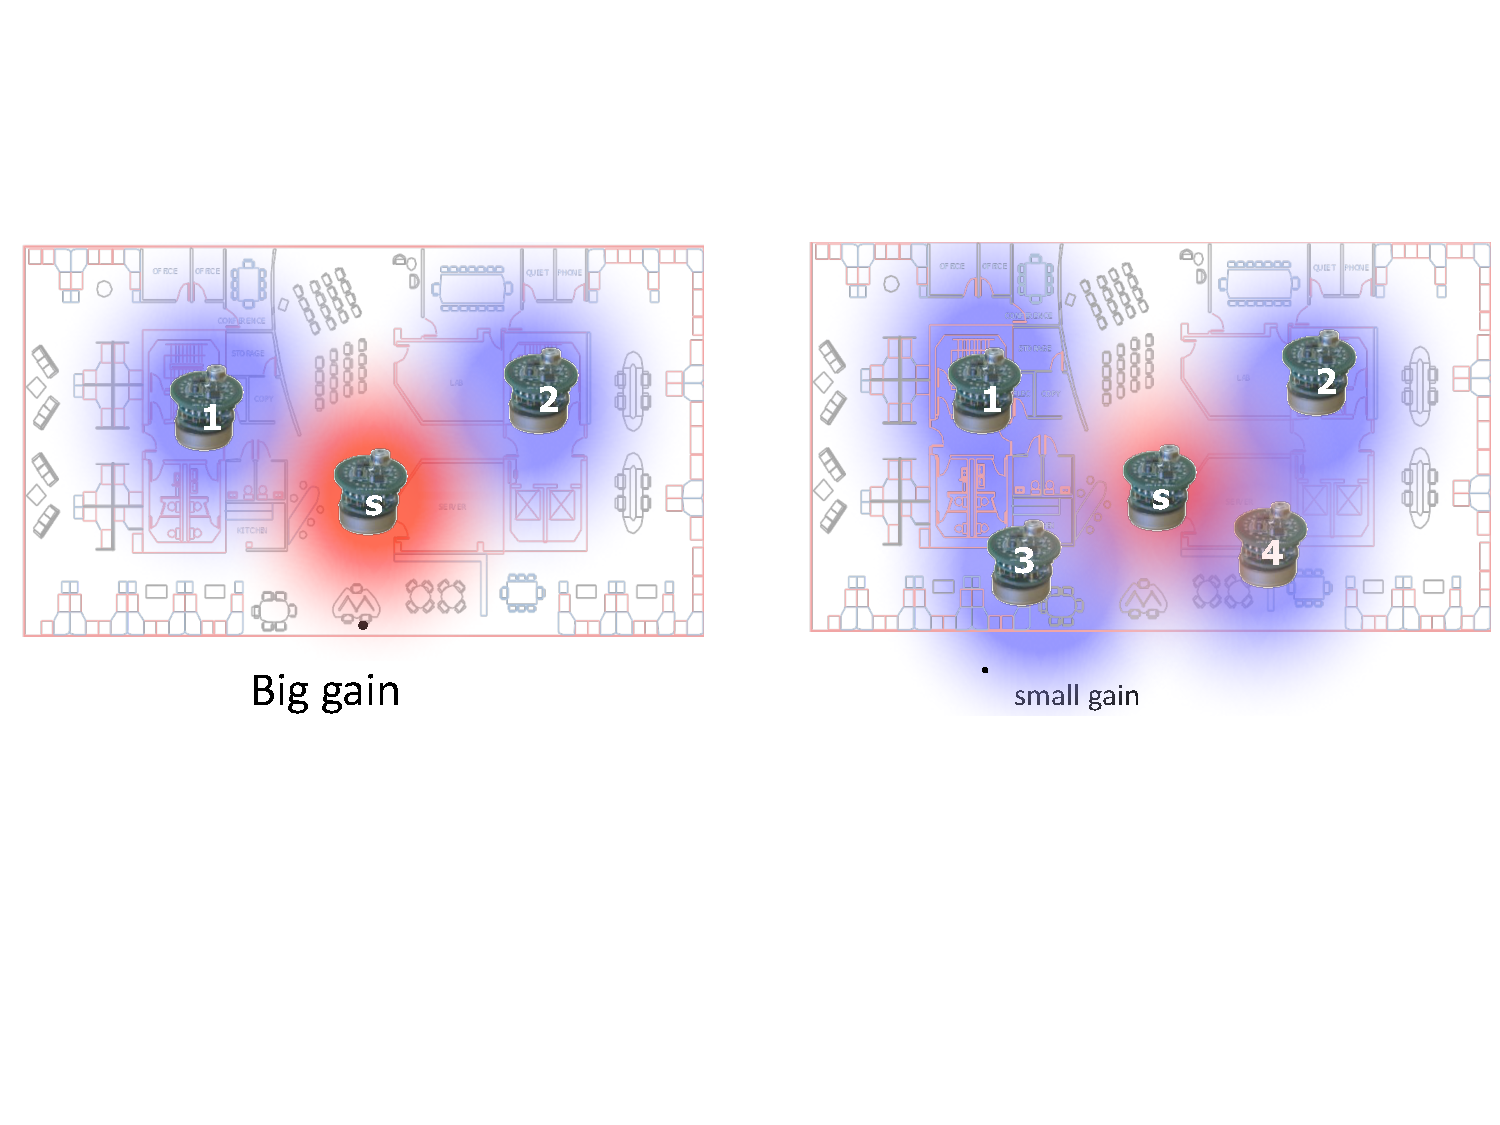
\includegraphics[scale=0.45]{diminishing_returns.pdf}
% \end{center}
% % \vspace{5pt}
% \textbf{Marginal value}: $f_{S}(B)= f(A \cup B)-f(A)$
% \end{frame}

% \begin{frame}{Submodular function Maximization} %Maximizing a submodular function?
% \begin{equation*}
%     \max_S f(S) \quad \text{ s.t.} \quad |S| \leq k - \text{cardinality constraint}
% \end{equation*}
% NP-hard in general.\\
% We consider $1 - 1/e - \varepsilon$ approximation of optimal solution $f^\star$.
% \end{frame}

\note{In recent years there has been a great deal of progress on fast algorithms for submodular maximization designed to accelerate computation on large data sets.}

\note{
The theoretical concept that captures the parallel time of an algorithm is adaptivity.
We say an algorithm is $r$-adaptive if it makes $r$ sequential rounds of parallel queries, where in each round it can make polynomialy many queries to a function evaluation oracle all at once.
So for example the familiar Greedy algorithm uses $k$ round to find a solution of $k$ elements. And in each round if you had polinomially many processors you could check of the remaining elements on a different processor to choose the best one in a single step. Therefore we say that greedy is $k$-adaptive. And note that $k$ is big Omega of n ($\Omega(n)$) in the worst case

Accelerating computation beyond linear runtime requires parallelization. The parallel runtime of blackbox optimization is measured by adaptivity, which is the number of sequential rounds an algorithm requires when polynomially-many queries can be executed in parallel in every round. 
For maximizing a submodular function defined over a ground set of n elements under a cardinality constraint k, the adaptivity of the naive greedy algorithm is O(k), which in the worst case is O(n).}

\begin{frame}{Parallel runtime = Adaptivity}
\begin{center}
    An algorithm is \textbf{$r$-adaptive} if it makes \\ $r$ sequential \textbf{rounds of parallel queries}.\vspace{5pt}
\centering
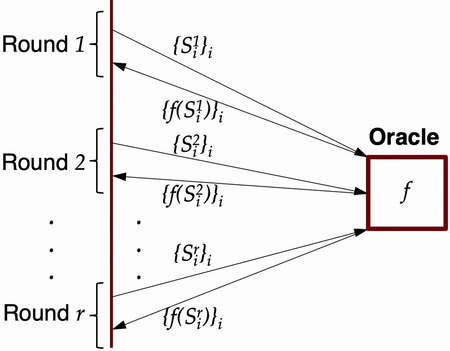
\includegraphics[scale=0.5]{adaptivity.png}
% \\
% \textbf{Adaptivity = parallel runtime}
\end{center}
The naive greedy algorithm adaptivity is $\mathcal{O}(k)$ for our problem.
% For maximizing a submodular function defined over a ground set of $n$ elements under a cardinality constraint $k$, the adaptivity of the naive greedy algorithm is $\cO(k)$
% adaptivity of the naive greedy algorithm is $\cO(k)$.
\end{frame}

\begin{frame}{Max-Cover Graph Problem} % Max-Cover problem
Given a graph $G$, the cover function $f(S)$ measures the count of nodes with at least one neighbor in $S$. This is a canonical monotone\footnote{$f$ is monotone if $A \subset B$ implies $f(A) \leq f(B)$} submodular function.
% We consider two algorithms for maximizing a monotone submodular function under a cardinality constraint $k$ and apply them to the graph Max Cover problem in particular.
\begin{figure}[t]
\begin{center}
\tikzset{every picture/.style={line width=0.75pt}} %set default line width to 0.75pt        
\begin{tikzpicture}[x=0.75pt,y=0.75pt,yscale=-1,xscale=1]
%uncomment if require: \path (0,300); %set diagram left start at 0, and has height of 300

%Shape: Circle [id:dp36255822406593574] 
\draw  [fill={rgb, 255:red, 0; green, 0; blue, 0 }  ,fill opacity=1 ] (98.21,120.31) .. controls (98.21,115.17) and (102.38,111) .. (107.52,111) .. controls (112.66,111) and (116.83,115.17) .. (116.83,120.31) .. controls (116.83,125.46) and (112.66,129.62) .. (107.52,129.62) .. controls (102.38,129.62) and (98.21,125.46) .. (98.21,120.31) -- cycle ;
%Straight Lines [id:da6762243021815164] 
\draw [line width=1.5]    (193.52,88.31) -- (107.52,120.31) ;
%Straight Lines [id:da5943065246596186] 
\draw [line width=1.5]    (193.52,88.31) -- (183.52,192.31) ;
%Straight Lines [id:da5922541880633836] 
\draw [line width=1.5]    (286.52,122.31) -- (193.52,88.31) ;
%Straight Lines [id:da5429713502318034] 
\draw [line width=1.5]    (286.52,122.31) -- (183.52,192.31) ;
%Straight Lines [id:da08272941688144808] 
\draw [line width=1.5]    (276.52,211.31) -- (183.52,192.31) ;
%Straight Lines [id:da7508692114128916] 
\draw [line width=1.5]    (352.52,183.31) -- (276.52,211.31) ;
%Straight Lines [id:da583686318615475] 
\draw [line width=1.5]    (286.52,122.31) -- (352.52,183.31) ;
%Shape: Ellipse [id:dp6095919685494009] 
\draw  [color={rgb, 255:red, 208; green, 2; blue, 27 }  ,draw opacity=1 ][line width=2.25]  (153.09,211.09) .. controls (142.55,195.02) and (170.68,157.93) .. (215.93,128.23) .. controls (261.18,98.53) and (306.41,87.47) .. (316.95,103.54) .. controls (327.49,119.6) and (299.36,156.7) .. (254.11,186.4) .. controls (208.86,216.1) and (163.64,227.15) .. (153.09,211.09) -- cycle ;
%Shape: Circle [id:dp6185527262442363] 
\draw  [fill={rgb, 255:red, 0; green, 0; blue, 0 }  ,fill opacity=1 ] (367.21,111.31) .. controls (367.21,106.17) and (371.38,102) .. (376.52,102) .. controls (381.66,102) and (385.83,106.17) .. (385.83,111.31) .. controls (385.83,116.46) and (381.66,120.62) .. (376.52,120.62) .. controls (371.38,120.62) and (367.21,116.46) .. (367.21,111.31) -- cycle ;
%Straight Lines [id:da2733414566463044] 
\draw [line width=1.5]    (352.52,183.31) -- (376.52,111.31) ;
%Shape: Circle [id:dp8390082539090082] 
\draw  [fill={rgb, 255:red, 208; green, 2; blue, 27 }  ,fill opacity=1 ] (174.21,192.31) .. controls (174.21,187.17) and (178.38,183) .. (183.52,183) .. controls (188.66,183) and (192.83,187.17) .. (192.83,192.31) .. controls (192.83,197.46) and (188.66,201.62) .. (183.52,201.62) .. controls (178.38,201.62) and (174.21,197.46) .. (174.21,192.31) -- cycle ;
%Shape: Circle [id:dp6411364120529555] 
\draw  [fill={rgb, 255:red, 208; green, 2; blue, 27 }  ,fill opacity=1 ] (277.21,122.31) .. controls (277.21,117.17) and (281.38,113) .. (286.52,113) .. controls (291.66,113) and (295.83,117.17) .. (295.83,122.31) .. controls (295.83,127.46) and (291.66,131.62) .. (286.52,131.62) .. controls (281.38,131.62) and (277.21,127.46) .. (277.21,122.31) -- cycle ;
%Shape: Circle [id:dp7676086263076403] 
\draw  [fill={rgb, 255:red, 74; green, 144; blue, 226 }  ,fill opacity=1 ] (184.21,88.31) .. controls (184.21,83.17) and (188.38,79) .. (193.52,79) .. controls (198.66,79) and (202.83,83.17) .. (202.83,88.31) .. controls (202.83,93.46) and (198.66,97.62) .. (193.52,97.62) .. controls (188.38,97.62) and (184.21,93.46) .. (184.21,88.31) -- cycle ;
%Shape: Circle [id:dp08773901760859015] 
\draw  [fill={rgb, 255:red, 74; green, 144; blue, 226 }  ,fill opacity=1 ] (267.21,211.31) .. controls (267.21,206.17) and (271.38,202) .. (276.52,202) .. controls (281.66,202) and (285.83,206.17) .. (285.83,211.31) .. controls (285.83,216.46) and (281.66,220.62) .. (276.52,220.62) .. controls (271.38,220.62) and (267.21,216.46) .. (267.21,211.31) -- cycle ;
%Shape: Circle [id:dp10937116699267224] 
\draw  [fill={rgb, 255:red, 74; green, 144; blue, 226 }  ,fill opacity=1 ] (343.21,183.31) .. controls (343.21,178.17) and (347.38,174) .. (352.52,174) .. controls (357.66,174) and (361.83,178.17) .. (361.83,183.31) .. controls (361.83,188.46) and (357.66,192.62) .. (352.52,192.62) .. controls (347.38,192.62) and (343.21,188.46) .. (343.21,183.31) -- cycle ;

% Text Node
\draw (332,96.4) node [anchor=north west][inner sep=0.75pt]    {$\textcolor{red}{S}$};
\end{tikzpicture}
% \tikzset{every picture/.style={line width=0.75pt}} %set default line width to 0.75pt        
% \begin{tikzpicture}[x=0.75pt,y=0.75pt,yscale=-1,xscale=1]
% %uncomment if require: \path (0,300); %set diagram left start at 0, and has height of 300

% %Shape: Circle [id:dp36255822406593574] 
% \draw  [fill={rgb, 255:red, 0; green, 0; blue, 0 }  ,fill opacity=1 ] (98.21,120.31) .. controls (98.21,115.17) and (102.38,111) .. (107.52,111) .. controls (112.66,111) and (116.83,115.17) .. (116.83,120.31) .. controls (116.83,125.46) and (112.66,129.62) .. (107.52,129.62) .. controls (102.38,129.62) and (98.21,125.46) .. (98.21,120.31) -- cycle ;
% %Straight Lines [id:da6762243021815164] 
% \draw [line width=1.5]    (193.52,88.31) -- (107.52,120.31) ;
% %Straight Lines [id:da5943065246596186] 
% \draw [line width=1.5]    (193.52,88.31) -- (183.52,192.31) ;
% %Straight Lines [id:da5922541880633836] 
% \draw [line width=1.5]    (286.52,122.31) -- (193.52,88.31) ;
% %Straight Lines [id:da5429713502318034] 
% \draw [line width=1.5]    (286.52,122.31) -- (183.52,192.31) ;
% %Straight Lines [id:da08272941688144808] 
% \draw [line width=1.5]    (276.52,211.31) -- (183.52,192.31) ;
% %Straight Lines [id:da7508692114128916] 
% \draw [line width=1.5]    (352.52,183.31) -- (276.52,211.31) ;
% %Straight Lines [id:da583686318615475] 
% \draw [line width=1.5]    (286.52,122.31) -- (352.52,183.31) ;
% %Shape: Ellipse [id:dp6095919685494009] 
% \draw  [color={rgb, 255:red, 208; green, 2; blue, 27 }  ,draw opacity=1 ][line width=2.25]  (153.09,211.09) .. controls (142.55,195.02) and (170.68,157.93) .. (215.93,128.23) .. controls (261.18,98.53) and (306.41,87.47) .. (316.95,103.54) .. controls (327.49,119.6) and (299.36,156.7) .. (254.11,186.4) .. controls (208.86,216.1) and (163.64,227.15) .. (153.09,211.09) -- cycle ;
% %Shape: Circle [id:dp6185527262442363] 
% \draw  [fill={rgb, 255:red, 0; green, 0; blue, 0 }  ,fill opacity=1 ] (367.21,111.31) .. controls (367.21,106.17) and (371.38,102) .. (376.52,102) .. controls (381.66,102) and (385.83,106.17) .. (385.83,111.31) .. controls (385.83,116.46) and (381.66,120.62) .. (376.52,120.62) .. controls (371.38,120.62) and (367.21,116.46) .. (367.21,111.31) -- cycle ;
% %Straight Lines [id:da2733414566463044] 
% \draw [line width=1.5]    (352.52,183.31) -- (376.52,111.31) ;
% %Shape: Circle [id:dp8390082539090082] 
% \draw  [fill={rgb, 255:red, 208; green, 2; blue, 27 }  ,fill opacity=1 ] (174.21,192.31) .. controls (174.21,187.17) and (178.38,183) .. (183.52,183) .. controls (188.66,183) and (192.83,187.17) .. (192.83,192.31) .. controls (192.83,197.46) and (188.66,201.62) .. (183.52,201.62) .. controls (178.38,201.62) and (174.21,197.46) .. (174.21,192.31) -- cycle ;
% %Shape: Circle [id:dp6411364120529555] 
% \draw  [fill={rgb, 255:red, 208; green, 2; blue, 27 }  ,fill opacity=1 ] (277.21,122.31) .. controls (277.21,117.17) and (281.38,113) .. (286.52,113) .. controls (291.66,113) and (295.83,117.17) .. (295.83,122.31) .. controls (295.83,127.46) and (291.66,131.62) .. (286.52,131.62) .. controls (281.38,131.62) and (277.21,127.46) .. (277.21,122.31) -- cycle ;
% %Shape: Circle [id:dp7676086263076403] 
% \draw  [fill={rgb, 255:red, 74; green, 144; blue, 226 }  ,fill opacity=1 ] (184.21,88.31) .. controls (184.21,83.17) and (188.38,79) .. (193.52,79) .. controls (198.66,79) and (202.83,83.17) .. (202.83,88.31) .. controls (202.83,93.46) and (198.66,97.62) .. (193.52,97.62) .. controls (188.38,97.62) and (184.21,93.46) .. (184.21,88.31) -- cycle ;
% %Shape: Circle [id:dp08773901760859015] 
% \draw  [fill={rgb, 255:red, 74; green, 144; blue, 226 }  ,fill opacity=1 ] (267.21,211.31) .. controls (267.21,206.17) and (271.38,202) .. (276.52,202) .. controls (281.66,202) and (285.83,206.17) .. (285.83,211.31) .. controls (285.83,216.46) and (281.66,220.62) .. (276.52,220.62) .. controls (271.38,220.62) and (267.21,216.46) .. (267.21,211.31) -- cycle ;
% %Shape: Circle [id:dp10937116699267224] 
% \draw  [fill={rgb, 255:red, 74; green, 144; blue, 226 }  ,fill opacity=1 ] (343.21,183.31) .. controls (343.21,178.17) and (347.38,174) .. (352.52,174) .. controls (357.66,174) and (361.83,178.17) .. (361.83,183.31) .. controls (361.83,188.46) and (357.66,192.62) .. (352.52,192.62) .. controls (347.38,192.62) and (343.21,188.46) .. (343.21,183.31) -- cycle ;

% % Text Node
% \draw (332,96.4) node [anchor=north west][inner sep=0.75pt]    {$\textcolor{red}{S}$};
% \end{tikzpicture}
\end{center}
\caption*{$f(\textcolor{red}{S}) = \textcolor{red}{2} + \textcolor{blue}{3} = 5$}
% \centering
\end{figure}
\vspace{-5pt}
% We maximize $f(S)$ to compare optimization algorithms. % $\max_{|S| \leq k} f(S)$
We solve problem $\max\limits_{|S| \leq k} f(S)$ to compare 2 optimization algorithms.
% Recent prior algorithms have comparable guarantees in terms of asymptotic worst case analysis, but their actual number of rounds and query complexity depend on very large constants and polynomials in terms of precision and confidence, making them impractical for large data sets.
\end{frame}

% \begin{frame}{Max cover on random graphs} % Problem Description
% Recall the max cover objective: given a graph $G$, the cover function $f(S)$ measures the count of nodes with at least one neighbor in $S$. This is a canonical monotone submodular function. To compare the algorithms’ runtimes under a range of conditions, we solve max cover on synthetic graphs generated via four different well-studied graph models:
% \emph{Stochastic Block Model} (SBM); \emph{Erd\H{o}s R\'{e}nyi} (ER); \emph{Watts-Strogatz} (WS); and \emph{Barb\'{a}si-Albert} (BA)
% % \begin{itemize}
% %     \item Erd˝os R´enyi. We generate $G(n, p)$ graphs with a $p = 0.01$ probability of each edge. Since many nodes have similar degree in this model and each node’s edges are spread randomly across the graph, a random set of nodes often achieves good coverage.
% %     \item Stochastic block model. We generate SBM graphs with a $p = 0.1$ probability of an edge between each pair of nodes in the same cluster. Here, we expect that a good solution will cover nodes in all clusters.
% %     \item Watts-Strogatz. We generate WS graphs initialized as ring lattices with 2 edges per node and a $p = 0.1$ probability of rewiring edges. In these ‘small-world’ graphs, many nodes have identical degree, so good solutions contain nodes chosen to minimize coverage overlaps.
% %     \item Barb´asi-Albert. We generate BA graphs with $m = 1$ edges added per iteration. BA graphs exhibit scale-free structure and tend to have a small set of high-degree nodes. Therefore, it is often possible to obtain high coverage in these graphs by choosing the highest degree nodes.
% % \end{itemize}

% \[\max _{|S| \leq k} \sum_{a \in S} f(a)\]
%     % Max cover on synthetic graphs generated via four different well-studied graph models: Stochastic Block Model (SBM); Erd˝os R´enyi (ER); Watts-Strogatz (WS); and Barb´asi-Albert (BA)
% \end{frame}

\begin{frame}{Algorithm 1: Randomized Parallel Greedy}
\begin{block}{The key steps:}
    \vspace{15pt}
\begin{itemize}
    \item We identify all “good” candidates with marginal values nearly as large as for the best elements.
    \vspace{15pt}
    \item We use a subset sampling $R \sim \delta S$ (where each element in S is drawn independently with probability $\delta$), and then we greedily choose $\delta$ as large as possible.
    \vspace{15pt}
    \item We sample  $R \sim \delta S$ with chosen probability $\delta$ and add it to the current set and update all variables accordingly.  
\end{itemize}
\end{block}

    
\end{frame}

\begin{frame}{Algorithm 1: Pseudo-code}

\begin{algorithm}[H]
\caption{Randomized Parallel Greedy}
  \label{greedy}
\begin{algorithmic}
\footnotesize
    	\STATE \textbf{input} function $f$, cardinality constraint $k$, parameter $\varepsilon$
\STATE$1 . Q \leftarrow \emptyset, t \leftarrow 0, \lambda \leftarrow \mathrm{OPT} $ (or any $\lambda \geq \mathrm{OPT}$)
\STATE $2.$ while $t \leq(1-2 \epsilon) k$ and $\lambda \geq e^{-1}$ OPT
\STATE \quad A. let $S=\left\{j \in N: f_{Q}(j) \geq \frac{(1-\epsilon) \lambda}{k}\right\}$ \quad \textbf{Finding "good" candidates}
\STATE \quad B. while $S$ is not empty and $t \leq(1-2 \epsilon) k$
\STATE \quad \quad i. choose $\delta$ maximal s.t.
\STATE \quad \quad \quad a. $F_{Q}(Q+\delta S) \geq(1-\epsilon)^{2} \lambda \frac{\delta|S|}{k}$\quad \textbf{We check expected marginal value}
\STATE \quad \quad \quad b. $t+\delta|S| \leq(1-2 \epsilon) k$\quad\quad\quad \quad  \textbf{We check cardinality constraint}
\STATE \quad \quad ii. sample $R \sim \delta S$
\STATE \quad \quad iii. $Q \leftarrow Q \cup R, t \leftarrow t+\delta|S|$\quad \quad \quad  \textbf{Updating variables}
\STATE \quad \quad iv. update $S$
\STATE \quad C. $\quad \lambda \leftarrow(1-\epsilon) \lambda$
\STATE $3.$ return $Q$
  \end{algorithmic}
\end{algorithm}
\end{frame}


\begin{frame}{Algorithm 2: Fast Adaptive Sequencing Technique (\textsc{Fast})} 
\textbf{Key Idea:} Uses adaptive sequencing with binary search over geometrically increasing indices of subsets.\\
\textbf{Adaptive Sequencing:}\\

\begin{center}
    {\includegraphics<1>[scale=0.25]{marginal_contributions.png}}
\end{center}
\end{frame}

\note{Another algorithm for solving the Max Cover problem is FAST, which stands for Fast Adaptive Sequencing Technique. And the key idea of this algorithm is an adaptive sequencing technique that uses binary search over geometrically increasing guesses of the optimal solution.

The idea behind adaptive sequencing is to generate a random sequence of nodes, and to search for some prefix by adding elements to some candidate prefix that gives a high marginal contribution when added to the a solution, S.}

\begin{frame}{Algorithm 2: Fast Adaptive Sequencing Technique (\textsc{Fast})}
\begin{center}
    {\includegraphics<1>[scale=0.25]{fast_full_2.png}}
\end{center}
\end{frame}
\note{In order to find nodes with high marginal contributions, FAST generates optimal guesses, V, with a geometric search over modular contributions of the nodes. And modularity here meaning, how many edges a single node can maximally contribute. And for each guess, it does a binary search to find the optimal set.

This search executes a subroutine, which uses adaptive sequencing to find a solution with high marginal contributions.}
\begin{frame}{Algorithm 2: Fast Adaptive Sequencing Technique (\textsc{Fast})}
\begin{center}
    {\includegraphics<1>[scale=0.25]{fast_partial.png}}
\end{center}
    \begin{itemize}
        \item Preprocess the input:
        \begin{itemize}
            \item Applies adaptive sequencing to find elements with high marginal contributions
            \item Discards the remaining elements with low marginal contributions.
        \end{itemize}
        \item Applies adaptive sequencing with binary searching over geometrically increasing prefixes on the remaining elements.

    \end{itemize}
\end{frame}
\note{The subroutine initializes an empty set S and until it meets the cardinality constraint of k nodes, it iteratively searches for a good solution. In each iteration, FAST has a preprocessing step, which generates a random sequence and selects the largest prefix that has a high marginal contribution to the current solution.

It then discards the remaining nodes in the set which have a low marginal contribution.

And finally, it applies adaptive sequencing on the remaining nodes by starting from the left and binary searching over geometrically increasing prefixes in which a large fraction of a sample of remaining nodes have high marginal value to the current solution. Denoted here by the union of the sequence prefix, A sub i-1, and the current solution S.

It then adds this sequence prefix A sub i to the current solution.
}
% \begin{frame}{Algorithm 2: Fast Adaptive Sequencing Technique (\textsc{Fast})} 
% \begin{algorithm}[H]
% \caption{\textsc{Fast-Full}: the full algorithm}
% \begin{algorithmic}
%     	\STATE \textbf{input} function $f$, cardinality constraint $k$, parameter $\varepsilon$
%     	\STATE $V \leftarrow$ \textsc{Geometric}$(\max_{a \in N} f(a), \max_{|S| \leq k} \sum_{a \in S} f(a), 1 - \varepsilon)$
%     	\STATE $v^{\star} \leftarrow$ \textsc{Binary-Search}$(V, \max\{v \in V: f(S_v) \geq (1 - 1/e)v\})$
%     	\STATE \ \ \ \ \ where $S_v \leftarrow$ \textsc{FAST}$(v)$
%     	\STATE \textbf{return} $S_{v^{\star}}$ 
%   \end{algorithmic}
%   \label{alg:full}
% \end{algorithm}
% \end{frame}

\begin{frame}{Theoretical guarantees}
% We show that \textsc{FAST} obtains a $1-1/e-\epsilon$ approximation w.p. $1- \delta$ and that it has $\tilde{O}(\varepsilon^{-2} \log n)$  adaptive complexity and $\tilde{O}(\varepsilon^{-2} n +\varepsilon^{-4} \log(n)  \log(\delta^{-1}))$ query complexity.
\begin{itemize}
    \item \footnotesize
    With prob. $1-\delta$, \textsc{\textbf{Randomized-Parallel-Greedy~[R-P-G]}} computes a $(1-\varepsilon)\left(1-e^{-1}\right)$ multiplicative approximation to the maximum value set of cardinality $k$ with $O\left(\frac{\log n}{\varepsilon^{2}}\right)$ expected adaptivity and $\tilde{O}\left(\frac{n}{\varepsilon^{4}}\right)$ expected oracle calls to $f$.
    \vspace{5pt}
    \item  \footnotesize
    Assume $k \geq \frac{2 \log(2\delta^{-1} \ell)}{\varepsilon^2 (1 - 5\varepsilon)}$ and $\varepsilon \in (0, 0.1)$, where  $\ell = \log(\frac{\log k}{\varepsilon})$. Then, \textsc{\textbf{FAST}} with $m = \frac{2 + \varepsilon}{\varepsilon^2(1 -  3\varepsilon)} \log(\frac{4\ell\log n}{\delta \varepsilon^2})$ has at most $\varepsilon^{-2} \log(n)  \ell^2$  adaptive rounds,    $2\varepsilon^{-2}  \ell n +  \varepsilon^{-2} \log(n) \ell^2 m$ queries, and achieves a $1 - \frac{1}{e} - 4 \varepsilon$ approximation w.p. $1 - \delta$.
\end{itemize}
% \begin{block}{Randomized-Parallel-Greedy [R-P-G]}
% \end{block}

% \begin{block}{FAST}
% \end{block}

% \begin{restatable}{rThm}{thmmain}
% \label{thm:main}
% Assume $k \geq \frac{2 \log(2\delta^{-1} \ell)}{\varepsilon^2 (1 - 5\varepsilon)}$ and $\varepsilon \in (0, 0.1)$, where  $\ell = \log(\frac{\log k}{\epsilon})$. Then, \algoptimized \ with $m = \frac{2 + \varepsilon}{\varepsilon^2(1 -  3\varepsilon)} \log(\frac{4\ell\log n}{\delta \varepsilon^2})$ has at most $\varepsilon^{-2} \log(n)  \ell^2$  adaptive rounds,   
% $2\varepsilon^{-2}  \ell n +  \varepsilon^{-2} \log(n) \ell^2 m$ queries, and achieves a $1 - \frac{1}{e} - 4 \varepsilon$ approximation 
% w.p. $1 - \delta$.
% \end{restatable}

\begin{columns}
    \column{\dimexpr\paperwidth-15pt}
    % \vspace{-15pt}
\begin{table}[h]
\begin{center}
\begin{tabular}{lllllll}%\vspace{0.2cm}
        & \emph{Query complexity} & \emph{Adaptivity} &   \\\ \vspace{0.5cm}
%  Randomized-Parallel-Greedy
 \textsc{R-P-G}& $\mathcal{O}\left(  \frac{n}{\varepsilon^4}  \log\left(\frac{n}{\delta}\right) \log^2 n\right)  $ & $ \mathcal{O}\left(\frac{\log n}{\varepsilon^2}  \right)$ & \\\ \vspace{0.3cm}
  \textsc{FAST} &     $\mathcal{O}\left(\frac{  n \ell}{\varepsilon^2} +  \frac{ \ell^2 \log n}{\epsilon^4}   \log(\frac{\ell\log n}{\delta \varepsilon^2})\right)$        &   $\mathcal{O}\left(\frac{ \ell^2 \log n}{\varepsilon^2}\right)$   & 
\end{tabular}
%   \caption{Comparison on the query complexity and adaptivity achieved in previous work and in this paper in order to obtain a $1-1/e-\epsilon$ approximation with probability $1 - \delta$, where  $\ell = \log(\frac{\log k}{\epsilon})$.  }
  \label{tab:queries}
\end{center}
\end{table}
\end{columns}
% $1-1/e-\epsilon$ approximation with probability $1 - \delta$
\end{frame}


\note{ FAST has a good approximation with high probability, 1-sigma, within the 1 - 1/e - epsilon approximation guarantee.
}

\begin{frame}{Experimental Setup}
We are going to 
\begin{itemize}
  \item Generate synthetic graphs as input to the Max Cover problem
    \begin{itemize}
        \item Stochastic Block Model (SBM)
        \item Erdos Renyi (ER)
        \item Watts-Strogatz (WS)
        \item Barbasi-Albert (BA)
    \end{itemize}
  \item Implement the Algorithms R-P-G and FAST in Python
  \item use Message Passing Interface (MPI) for parallelization since it gives precise control over the parallel communication between processors
  \item Run the algorithms on CPU nodes provided by KAUST Ibex Cluster

\end{itemize}

\end{frame}

\begin{frame}{Software Creation Plan}
\begin{tabular}{||c c||} 
 \hline
 Date & Tasks \\
 \hline\hline
 2-8 November & Implement Synthetic Graph Generation  \\ 
 \hline
 9-15 November & Implement Randomized-Parallel-Greedy \\
 \hline
 16-22 November & Implement FAST algorithm  \\
 \hline
 23-29 November & Setup Ibex environment and Debug  \\
 \hline
 1-7 December & Run experiments and obtain results  \\
 \hline
 8-13 December & Prepare for project report and presentation  \\
 \hline
\end{tabular}
\end{frame}

\begin{frame}{References}
\tiny % \small
\begin{thebibliography}{99}
    \bibitem[NW78]{nemhauser1978best} George~L Nemhauser and Laurence~A Wolsey.
	\newblock Best Algorithms for Approximating the Maximum of a Submodular Set Function.
	\newblock {\em Mathematics of operations research}, 3(3):177--188, 1978.
	
    \bibitem[CQ19b]{chekuri2018submodular} Chandra Chekuri and Kent Quanrud.
	\newblock Submodular Function Maximization in Parallel via the Multilinear Relaxation.
	\newblock \emph{Proceedings of the 2019 Annual ACM-SIAM Symposium on Discrete Algorithms, 2019}

    \bibitem[Breuer et al, 2020]{breuer2019fast} A. Breuer, E. Balkanski, and Y. Singer
	\newblock The FAST Algorithm for Submodular Maximization.
	\newblock \emph{Proceedings of the 37th International Conference on Machine Learning, 2020.}
	
	\bibitem[BRS19b]{BRS19b} Eric Balkanski, Aviad Rubinstein, and Yaron Singer.
	\newblock An optimal approximation for submodular maximization under a matroid constraint in the adaptive complexity model.
	\newblock {\em STOC}, 2019.
	
% 	\bibitem[Liu et al, 2020]{liu_fedsel_2020} R. Liu, Y. Cao, M. Yoshikawa, and H. Chen.
% 	\newblock FedSel: Federated SGD under Local Differential Privacy with Top-k Dimension Selection.
% 	\newblock \emph{Foundations and Trends in Theoretical Computer Science, 9(3–4):211–407, 2014.}
\end{thebibliography}
\end{frame}

\end{document}
